\chapter{Un poco de historia}

Windows Server es la línea de productos de Microsoft \textbf{enfocada a servidores} que se inició con la primera versión: Windows 2000.

Anteriormente, Microsoft contaba con una línea también dedicada a estaciones de trabajo y servidores en red cuyo nombre era Windows NT, por lo que se puede considerar que \textbf{Windows Server es la continuación de NT} con el cambio de nombre.

Las versiones más importantes han sido, sin contar las denominadas NT:
\begin{itemize}
    \item Windows 2000.
    \item Windows Server 2003.
    \item Windows Server 2008.
    \item Windows Server 2012.
    \item Windows Server 2016.
    \item Windows Server 2019.
\end{itemize}

\chapter{Proceso de instalación de Windows Server 2019}
Para realizar la instalación de Windows Server 2019 necesitaremos el medio desde el que realizaremos la instalación. Microsoft permite la descarga desde su página oficial una evaluación de 180 días que podremos descargar en varios formatos:

\begin{itemize}
    \item \textbf{Azure}: Es el sistema “en la nube” de Microsoft. Se puede probar Windows Server a través de una cuenta gratuita y posteriormente gestionar los sistemas virtualizados que se creen en la nube.
    \item \textbf{ISO}: Una imagen ISO que podremos utilizar grabándolo en un DVD, a través de un USB o usarlo en un sistema de virtualización propio.
    \item \textbf{VHD}: Formato de archivo que representa una unidad de disco duro virtual.
\end{itemize}

Para realizar una instalación completa en nuestro sistema de virtualización elegiremos el archivo ISO. Para poder descargarlo tendremos que rellenar un formulario, elegir el idioma y posteriormente comenzará la descarga.

\section{Requisitos previos}
Antes de realizar la instalación debemos conocer cuáles son los requisitos mínimos de hardware que necesita Windows Server para así asegurar que la máquina virtual (o el hardware donde lo vamos a instalar) es 100\% compatible. En este caso, y tal como nos indica la web de Microsoft, los requisitos son:

\begin{itemize}
    \item \textbf{Procesador} de 64 bits a 1,4 GHz, compatible con el conjunto de instrucciones x64
    \begin{itemize}
        \item Admite DEP y NX
        \item Admite CMPXCHG16b, LAHF/SAHF y PrefetchW
        \item Admite la traducción de direcciones de segundo nivel (EPT o NPT)
    \end{itemize}
    \item \textbf{RAM}: 512 MB (\textbf{2 GB} para la opción de instalación Servidor con Experiencia de escritorio). Se admite RAM tipo ECC (código de corrección de errores)
    \item \textbf{Espacio en disco}:  mínimo 32GB. Windows Server no admite discos ATA, PATA, IDE y EIDE para unidades de arranque, página o datos.
    \item \textbf{Adaptador de red} de 1 gigabit/s
\end{itemize}

Dado que estos son los requisitos mínimos, nuestra máquina virtual deberá cumplirlos, pero en un sistema que vaya a estar en producción deberemos realizar un análisis de requisitos para asegurar que el hardware (ya sea virtual o físico) cumple las necesidades de los servicios que alojará:

\begin{itemize}
    \item ¿El servidor va a contar con un servidor web?
    \begin{itemize}
        \item ¿Cuántas visitas se esperan?
        \item ¿Qué tipo de web va a servir? ¿Programada en Java, PHP, …?
    \end{itemize}
    \item ¿El servidor va a contar con un sistema gestor de base de datos?
    \begin{itemize}
        \item ¿Cuántas bases de datos va a tener?
        \item ¿Cuántas conexiones simultáneas esperamos?
        \item ¿Cuántas peticiones estimamos que va a recibir?
    \end{itemize}
    \item ¿El servidor va a servir para compartir ficheros?
    \begin{itemize}
        \item ¿Cuántos usuarios van a acceder?
        \item ¿Peticiones estimadas?
    \end{itemize}
    \item …
\end{itemize}

Por tanto, antes de realizar la instalación, deberemos confirmar que conocemos para qué se va a utilizar el servidor, cuántos servicios se van a utilizar y la carga esperada.

\section{Instalación de Windows Server 2019}
El asistente de instalación de Windows Server nos va a llevar por una serie de pasos que detallaremos a continuación.
\warnbox{Nos aseguramos que la máquina virtual arranque desde la ISO}

\subsection{Elección del idioma}
El primer paso del asistente será elegir el idioma principal que usaremos en el sistema operativo. Antes de realizar la descarga de la ISO hemos elegido el idioma español, por lo que el asistente nos aparecerá por defecto en ese idioma. Podremos elegir:

\begin{itemize}
    \item Idioma que va a instalar
    \item Formato de hora y moneda
    \item Teclado o método de entrada
\end{itemize}

En nuestro caso dejaremos las opciones tal como nos aparece por defecto, pero de utilizar el servidor en un sistema internacional, convendría hacer uso del sistema en inglés.

\subsection{Elección del sistema operativo}
Windows Server 2019 tiene distintos modos a la hora de ser instalado, tal como podemos ver en la siguiente captura de pantalla del proceso de instalación:
\begin{center}
  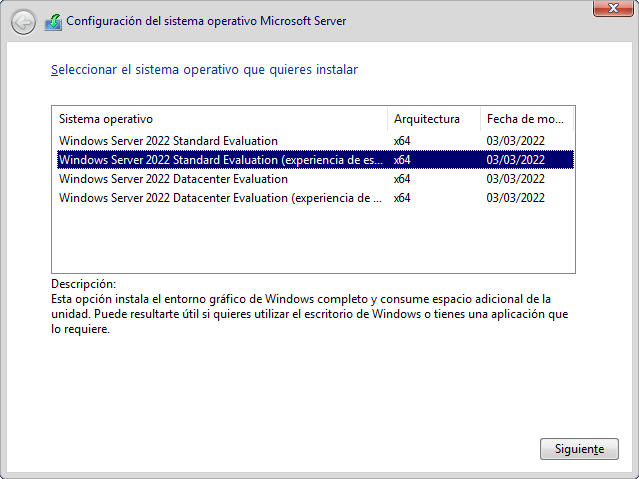
\includegraphics[width=14cm]{2_instalacion.png}
\end{center}

Existen dos opciones principales a la hora de elegir, ya que cada una de ellas permitirá instalarlo con o sin experiencia de escritorio. Las opciones principales son:

\begin{itemize}
    \item \textbf{Standard Evaluation}: Útil para empresas medianas o pequeñas, que no requieran de grandes sistemas de virtualización.
    \item \textbf{Datacenter Evaluation}: No habrá límite a la hora de crear máquinas virtuales con un host Hyper-V por cada licencia.
\end{itemize}

Existen más diferencias, y es por eso que Microsoft tiene una página dedicada con la \href{https://docs.microsoft.com/es-es/windows-server/get-started/editions-comparison-windows-server-2019}{comparación de ambas versiones}. Por lo tanto, antes de realizar la instalación para nuestro sistema, debemos realizar una estimación de los requisitos para así poder elegir de manera adecuada.

Nosotros vamos a elegir la versión “Standard Evaluation” con experiencia de escritorio ya que podremos realizar la configuración desde el propio servidor. Dependiendo del caso, habrá que analizar cuál es la mejor opción antes de realizar la instalación.

Al darle a “Siguiente” nos aparecerán los términos de la licencia.

\subsection{Tipo de instalación}
Tras aceptar la licencia nos aparecerá el tipo de instalación que deseamos realizar:
\begin{center}
  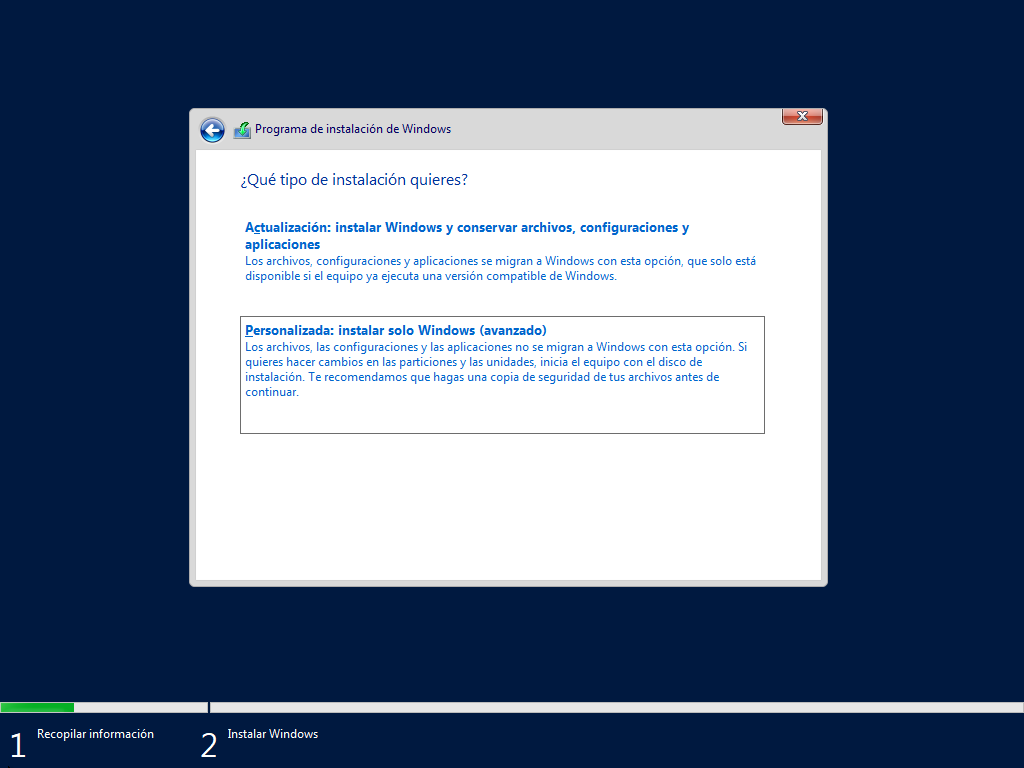
\includegraphics[width=14cm]{3_instalacion.png}
\end{center}

\begin{itemize}
    \item \textbf{Actualización}: Para realizar actualizaciones sobre sistemas compatibles ya instalados.
    \item \textbf{Personalizada}: Tal como indica la imagen anterior, los archivos, las configuraciones y las aplicaciones no se migran. En caso de realizar una instalación nueva (como en nuestro caso), \textbf{utilizaremos esta opción}.
\end{itemize}

\subsection{Particionado de discos duros}
Dado que nuestra máquina virtual es nueva, y no tiene ningún sistema operativo previo, vamos a tener que realizar la instalación en el disco duro que se ha añadido a la máquina virtual.

Dependiendo del tamaño que hayamos elegido, o incluso los discos duros que tengamos, nos aparecerán en la nueva pantalla del programa de instalación.

En nuestro caso la máquina virtual cuenta con un único disco duro de 40GB de almacenamiento, en donde realizaremos la instalación de la manera predeterminada que Windows Server elija particionarlo. Por lo tanto, seleccionaremos el disco duro y le daremos al botón de “Siguiente”.



